\documentclass[notes,10pt, aspectratio=169]{beamer}

\usepackage{pgfpages}
% These slides also contain speaker notes. You can print just the slides,
% just the notes, or both, depending on the setting below. Comment out the want
% you want.
\setbeameroption{hide notes} % Only slide
%\setbeameroption{show only notes} % Only notes
%\setbeameroption{show notes on second screen=right} % Both

\usepackage{helvet}
\usepackage[default]{lato}
\usepackage{array}
\usepackage{eurosym}
\usepackage{setspace}
\usepackage{animate}
\usepackage{multicol}
\usepackage{breqn}
\usepackage{subcaption}
\usepackage{caption}
\captionsetup{font=scriptsize, justification=raggedright,singlelinecheck=false}
\usepackage[export]{adjustbox}
\usepackage[scale=2]{ccicons}
\usepackage{tikz}
\newenvironment{wideitemize}{\itemize\addtolength{\itemsep}{10pt}}{\enditemize}
\usepackage{natbib}

\usepackage{tikz}
\usepackage{verbatim}
\setbeamertemplate{note page}{\pagecolor{yellow!5}\insertnote}
\usepackage{amsmath}
%\usepackage{mathpazo}
\usepackage{hyperref}
\usepackage{lipsum}
\usepackage{multimedia}
\usepackage{multirow}
\usepackage{graphicx}
\usepackage{dcolumn}
\usepackage{bbm}
\newcolumntype{d}[0]{D{.}{.}{5}}

\usepackage{changepage}
\usepackage{appendixnumberbeamer}
% \newcommand{\beginbackup}{
%   \newcounter{framenumbervorappendix}
%   \setcounter{framenumbervorappendix}{\value{framenumber}}
%   \setbeamertemplate{footline}
%   {
%      \leavevmode%
%      \hline
%      box{%
%       \begin{beamercolorbox}[wd=\paperwidth,ht=2.25ex,dp=1ex,right]{footlinecolor}%
% %         \insertframenumber  \hspace*{2ex} 
%       \end{beamercolorbox}}%
%      \vskip0pt%
%   }
%  }

 \setbeamertemplate{footline}{
    \hbox{%
    \begin{beamercolorbox}[wd=\paperwidth,ht=3ex,dp=1.5ex,leftskip=2ex,rightskip=2ex]{page footer}%
        %\usebeamerfont{title in head/foot}%
        %\insertshorttitle \hfill
        %\insertsection \hfill
        %\tableofcontents[currentsection] \hfill
        \insertsectionnavigationhorizontal{0.7\paperwidth}{}{} \hfill 
        \insertframenumber{} / \inserttotalframenumber
    \end{beamercolorbox}}%
}
\newcommand{\backupend}{
   \addtocounter{framenumbervorappendix}{-\value{framenumber}}
   \addtocounter{framenumber}{\value{framenumbervorappendix}} 
}


\usepackage{graphicx}
\usepackage[space]{grffile}
\usepackage{booktabs}

% These are my colors -- there are many like them, but these ones are mine.
\definecolor{blue}{RGB}{0,114,178}
\definecolor{red}{RGB}{213,94,0}
\definecolor{yellow}{RGB}{240,228,66}
\definecolor{green}{RGB}{0,158,115}

\setbeamercolor{section in head/foot}{fg=blue}

\useinnertheme[shadow]{rounded}
\setbeamercolor{block title example}{fg=black,bg=orange!50!white}
\setbeamercolor{block body example}{fg=black, bg=orange!30!white}


\hypersetup{
  colorlinks=false,
  linkbordercolor = {white},
  linkcolor = {blue}
}


%% I use a beige off white for my background
\definecolor{MyBackground}{RGB}{255,253,218}

%% Uncomment this if you want to change the background color to something else
%\setbeamercolor{background canvas}{bg=MyBackground}

%% Change the bg color to adjust your transition slide background color!
\newenvironment{transitionframe}{
  \setbeamercolor{background canvas}{bg=yellow}
  \begin{frame}}{
    \end{frame}
}

\setbeamercolor{frametitle}{fg=blue}
\setbeamercolor{title}{fg=black}
%\setbeamertemplate{footline}[frame number]
\setbeamertemplate{navigation symbols}{} 
\setbeamertemplate{itemize items}{-}
\setbeamercolor{itemize item}{fg=blue}
\setbeamercolor{itemize subitem}{fg=blue}
\setbeamercolor{enumerate item}{fg=blue}
\setbeamercolor{enumerate subitem}{fg=blue}
\setbeamercolor{button}{bg=white,fg=blue,}



% If you like road maps, rather than having clutter at the top, have a roadmap show up at the end of each section 
% (and after your introduction)
% Uncomment this is if you want the roadmap!
% \AtBeginSection[]
% {
%    \begin{frame}
%        \frametitle{Roadmap of Talk}
%        \tableofcontents[currentsection]
%    \end{frame}
% }
\setbeamercolor{section in toc}{fg=blue}
\setbeamercolor{subsection in toc}{fg=red}
%\setbeamersize{text margin left=1em,text margin right=1em} 
\setbeamersize{text margin left=0.7cm,text margin right=0.7cm} 


\title[]{\textcolor{blue}{Practice 2:\\OLS and the RAND Experiment}}
\author{25117 - Econometrics}
\institute[shortinst]{Universitat Pompeu Fabra}

\date{October 14th, 2024}

\begin{document}


% Title Slide

\begin{frame}[plain]
\maketitle
\end{frame}

\begin{frame}
\frametitle{Introduction to Ordinary Least Squares (OLS)}
\begin{itemize}
    \item Ordinary Least Squares (OLS) is a fundamental statistical technique used in linear regression analysis.\\\\[1em]
    \item It seeks to determine the best-fitting linear relationship between a dependent variable (e.g., earnings) and one or more independent variables (e.g., working hours)...\\\\[1em]
    \item ...by minimizing the sum of squared differences between observed and predicted values.\\\\[1em]
    \begin{itemize}
        \item \textbf{Example:} Consider a young researcher who wants to understand the relationship between their monthly earnings and the number of hours worked each week. OLS helps in finding the linear relationship between earnings and working hours.\\\\[1em]
    \end{itemize}
\end{itemize}

\begin{exampleblock}{Question}
    What are the two primary objectives of researchers when fitting a regression line?
\end{exampleblock}
\end{frame}

\begin{frame}
\frametitle{The Regression Line}

\begin{itemize}
    \item  The regression line, often represented as $Y = aX + b$, is the central output of OLS.\\\\[1em]
    \item In this equation, $Y$ represents the dependent variable (e.g., earnings), $X$ represents the independent variable (e.g., working hours), and $a$ and $b$ are coefficients to be estimated by OLS.\\\\[1em]
    \begin{itemize}
        \item \textbf{Example:} For instance, if the OLS analysis suggests the equation $Earnings = 15 \times Hours + 100$ it implies that for every additional hour worked, earnings are expected to increase by \$15. The starting point for earnings, even with no hours worked, is \$100.
    \end{itemize}
\end{itemize}

\begin{exampleblock}{Question}
In the equation $Y = aX + b$, what does the coefficient 'a' represent, and what does 'b' signify?
\end{exampleblock}

\end{frame}

\begin{frame}
\frametitle{Residuals and Minimizing Squared Errors}

\begin{itemize}
    \item  Residuals are the discrepancies between actual observed values (e.g., actual earnings) and the values predicted by the regression line.\\\\[1em]
    \item OLS minimizes the sum of squared residuals, effectively striving to minimize these differences.\\\\[1em]
    \begin{itemize}
        \item \textbf{Example:} Suppose the regression model predicts earnings of \$300 for 20 hours worked, but the actual earnings are \$280. In this case, the residual is \$280 - \$300 = -\$20.
    \end{itemize}
\end{itemize}

\begin{exampleblock}{Question}
What are residuals, how to interpret them, and how does OLS utilize them to find the best-fit linear relationship?
\end{exampleblock}

\end{frame}

\begin{frame}
\frametitle{Goodness-of-Fit}
\begin{itemize}
    \item  The R-squared, or $R^2$ is a statistical measure that assesses the goodness of fit of a regression model.\\\\[1em]
    \item It quantifies the proportion of variance in the dependent variable (e.g., earnings) that is explained by the independent variable(s) (e.g., working hours) in the model.\\\\[1em]
    \item R-squared values range from 0 (no fit) to 1 (perfect fit).\\\\[1em]
    \begin{itemize}
        \item \textbf{Example:} If your earnings and working hours model has an R-squared value of 0.75, it signifies that 75\% of the variability in earnings can be attributed to the number of hours worked.
    \end{itemize}
\end{itemize}

\begin{exampleblock}{Question}
Is a high $R^2$ an indicator of a strong causal relationship between the independent and dependent variables?
\end{exampleblock}

\end{frame}

\begin{frame}
\frametitle{Limitations of OLS}
\begin{itemize}
    \item Although OLS is a powerful and widely used tool, it has limitations.\\\\[1em]
    \item E.g., it assumes a linear relationship between variables, which may not hold in all cases.\\\\[1em]
    \item Additionally, OLS can be sensitive to outliers, which are extreme data points that can unduly influence the model's accuracy.\\\\[1em]
 \begin{itemize}
        \item \textbf{Example:} Consider a case where an individual received an unusually large bonus due to exceptional performance in one month. OLS might not handle this outlier well, potentially leading to inaccurate future earnings predictions, as it inherently assumes a linear relationship.
    \end{itemize}
\end{itemize}

\begin{exampleblock}{Question}
 What are the OLS assumptions, and how do they affect the interpretation of your results?
\end{exampleblock}

\end{frame}

\begin{frame}
\frametitle{The Impact of Healthcare Insurance on Medical Spending}
Healthcare insurance can significantly influence medical spending...\\\\[1em]

\begin{enumerate}
  \item \textbf{Moral Hazard}:
    \begin{itemize}
      \item Insured individuals may seek more medical care due to reduced financial burden, potentially increasing medical costs.\\\\[1em]
    \end{itemize}

  \item \textbf{Price Sensitivity}:
    \begin{itemize}
      \item Well-insured patients may not closely examine or negotiate healthcare costs, leading to higher prices in the healthcare industry.\\\\[1em]
    \end{itemize}

  \item \textbf{Provider Behavior}:
    \begin{itemize}
      \item When patients have insurance, providers may order more tests and treatments to maximize revenue, increasing healthcare expenses.\\\\[1em]
    \end{itemize}

  % \item \textbf{Government Intervention}:
  %   \begin{itemize}
  %     \item Public policies and regulations can shape the extent of insurance coverage, reimbursement rates, and overall healthcare spending.\\\\[1em]
  %   \end{itemize}
\end{enumerate}
\end{frame}

\begin{frame}
\frametitle{Balancing Act - Healthcare Insurance and Medical Spending}
However, healthcare insurance also plays a complex role in the economic ecosystem, with numerous positive aspects.\\\\[1em]

\begin{enumerate}
  \item \textbf{Risk Pooling}:
    \begin{itemize}
      \item Insurance provides risk pooling benefits, spreading the cost of expensive treatments across a larger group of policyholders, reducing the financial burden of catastrophic health events for individuals.\\\\[1em]
    \end{itemize}

  \item \textbf{Preventive Care}:
    \begin{itemize}
      \item Health insurance encourages individuals to seek preventive care and early treatment for health issues, potentially reducing the overall cost of healthcare by avoiding more expensive treatments down the road.\\\\[1em]
    \end{itemize}

  \item \textbf{Innovation and Technology}:
    \begin{itemize}
      \item Health insurance influences the development and adoption of new medical technologies and drugs. Insured patients are more likely to use advanced and expensive treatments, driving innovation but also contributing to rising healthcare costs.\\\\[1em]
    \end{itemize}

%   \item \textbf{Government Policies}:
%     \begin{itemize}
%       \item Government policies significantly shape healthcare insurance and spending and can determine the effectiveness of healthcare systems.\\\\[1em]
%     \end{itemize}
\end{enumerate}
\end{frame}

\begin{frame}{In Practice: Healthcare Insurance vs. Medical spendings}
\begin{itemize}
    \item The government charges you to understand the impact of extended healthcare insurance on medical spending.
    \item There is no normative aspect in the question (i.e., is healthcare good or bad), just a positive one (i.e., quantify the impact).
\end{itemize}

    \begin{exampleblock}{Questions}
    \begin{itemize}
        \item What would you expect from the theory?
        \item What would be the gold standard experiment that would allow you to answer this question?
        \item How would you proceed?
        \item In practice, what challenges would you face?
    \end{itemize}
    \end{exampleblock}
\end{frame}


\begin{frame}{The RAND Health Insurance Experiment}
  \begin{itemize}
    \item The RAND experiment was a groundbreaking study conducted between 1974 and 1981.\\\\[1em]
    \item \textbf{Objective}: To assess the impact of different health insurance plans on medical spending and health outcomes.\\\\[1em]
    \item \textbf{Methodology}: Randomized controlled trial with over 5,800 individuals in 2,750 families.\\\\[1em]
    \item \textbf{Insurance Plans}: Participants were randomly assigned to 6 different insurance plans for 3 to 5 years:
      \begin{itemize}
        \item \textbf{4 different copayments plans}: 0, 25, 50, 95\%
        \item \textbf{1 mixed plan}: 25\% in general \& 50\% for dental and outpatient services
        \item \textbf{1 individually deductible}: 95\%  outpatient and 0\% inpatient services
      \end{itemize}\\\\[1em]
    \item \textbf{Key Findings}:
      \begin{itemize}
        \item \textbf{Moral Hazard}: Those with free care consumed more healthcare services, leading to higher costs.
        \item \textbf{Health Outcomes}: No significant differences in health outcomes between plans.
        \item \textbf{Cost-Sharing Effect}: Plans with cost-sharing reduced medical spending, but at the expense of decreased utilization of necessary care.
      \end{itemize}
  \end{itemize}

\end{frame}


\begin{frame}{Descriptive Stats}
    \begin{center}
        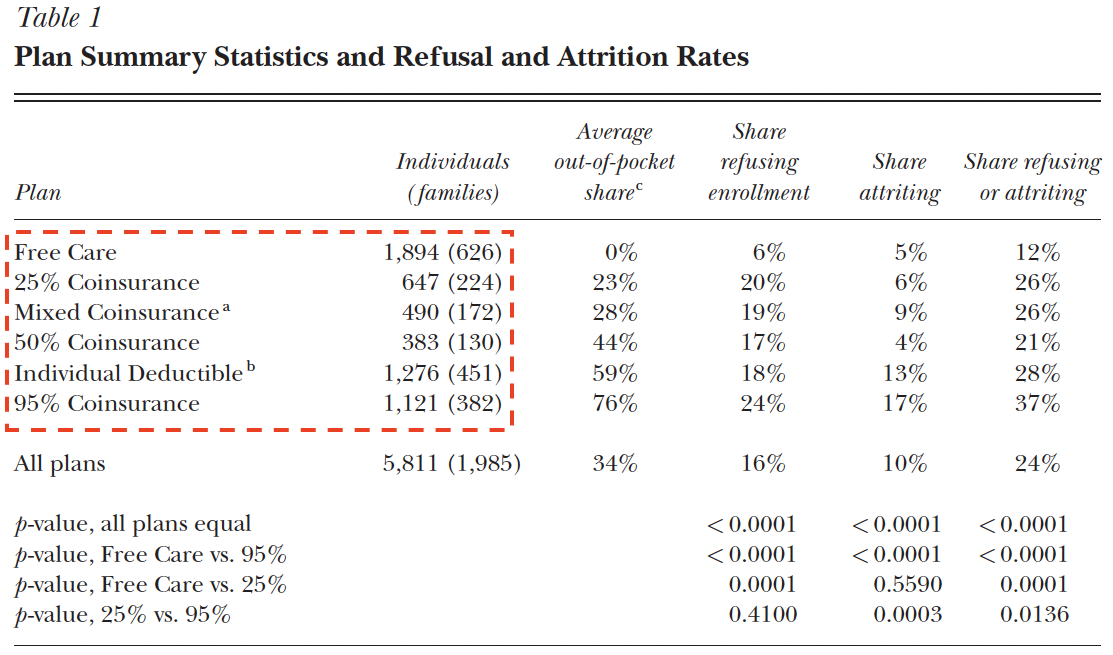
\includegraphics[scale=.53]{images/rand0.png}
    \end{center}
\end{frame}

\begin{frame}{Descriptive Stats}
    \begin{center}
        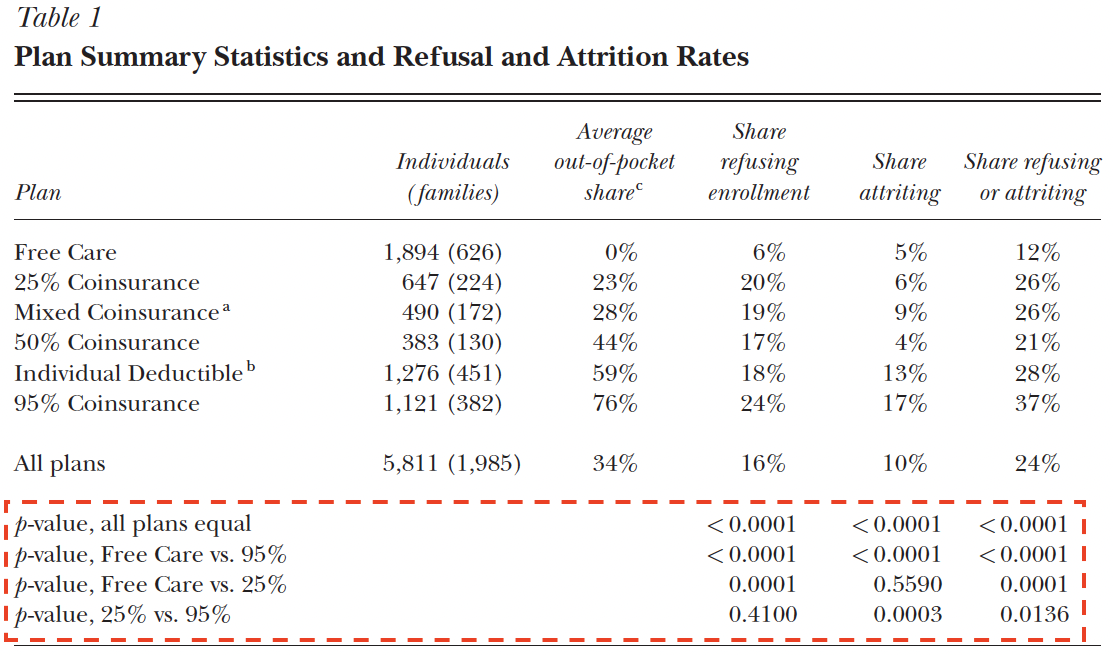
\includegraphics[scale=.53]{images/rand1.png}
    \end{center}
\end{frame}

\begin{frame}{Main Results}
    \begin{center}
        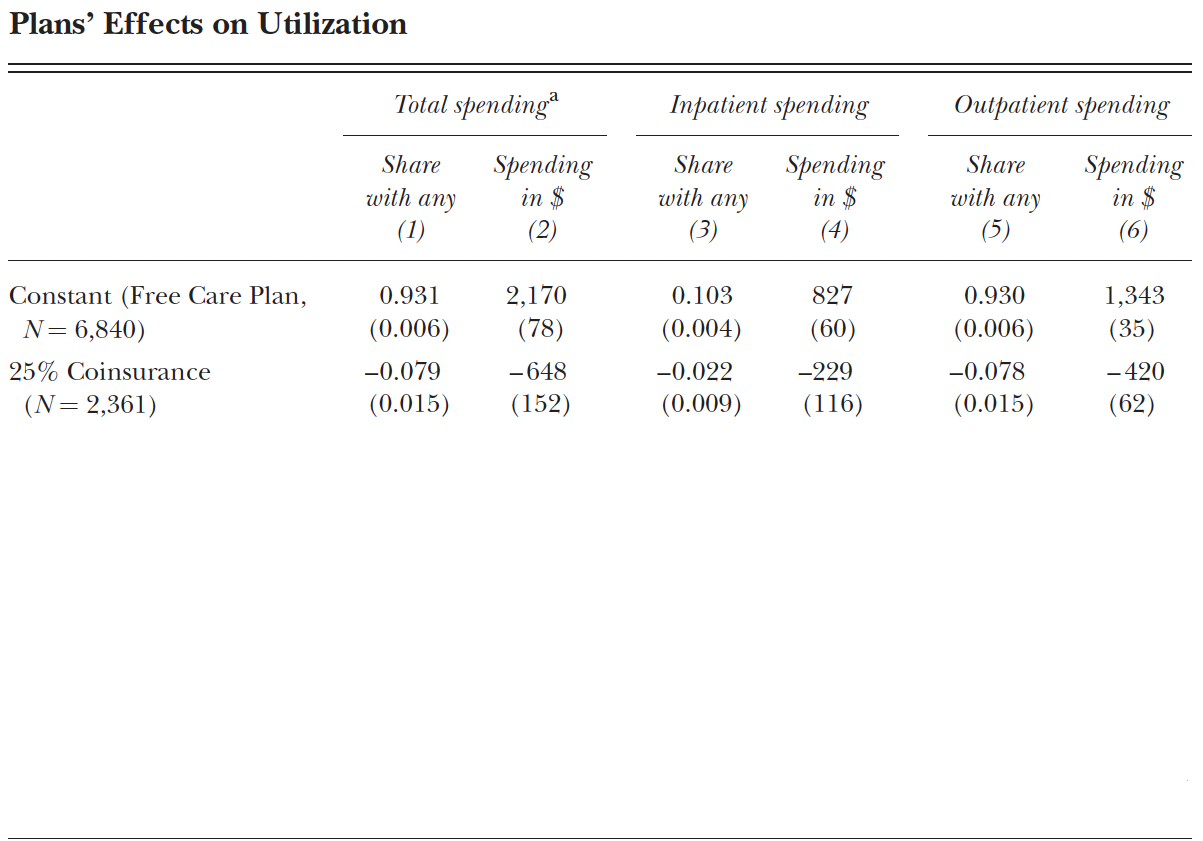
\includegraphics[scale=.53]{images/rand2.png}
    \end{center}
\end{frame}

\begin{frame}{Main Results}
    \begin{center}
        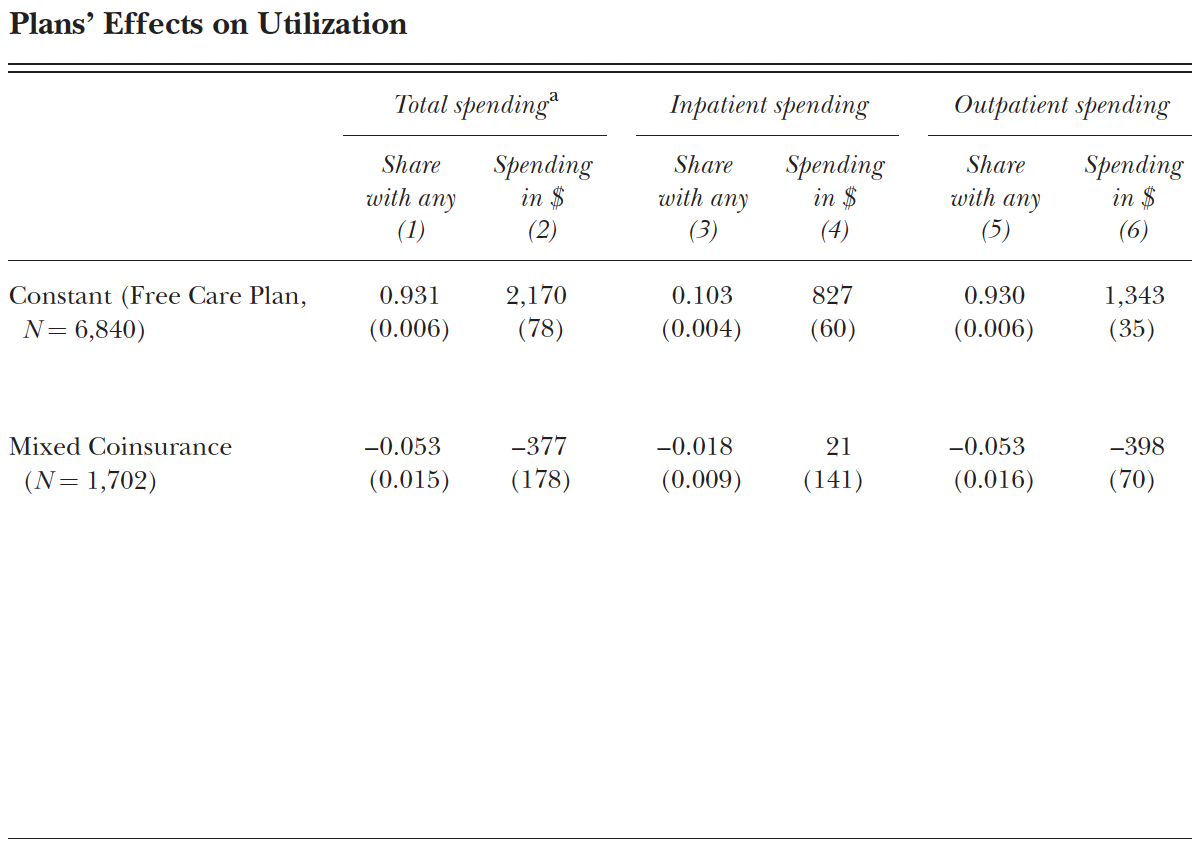
\includegraphics[scale=.53]{images/rand3.png}
    \end{center}
\end{frame}

\begin{frame}{Main Results}
    \begin{center}
        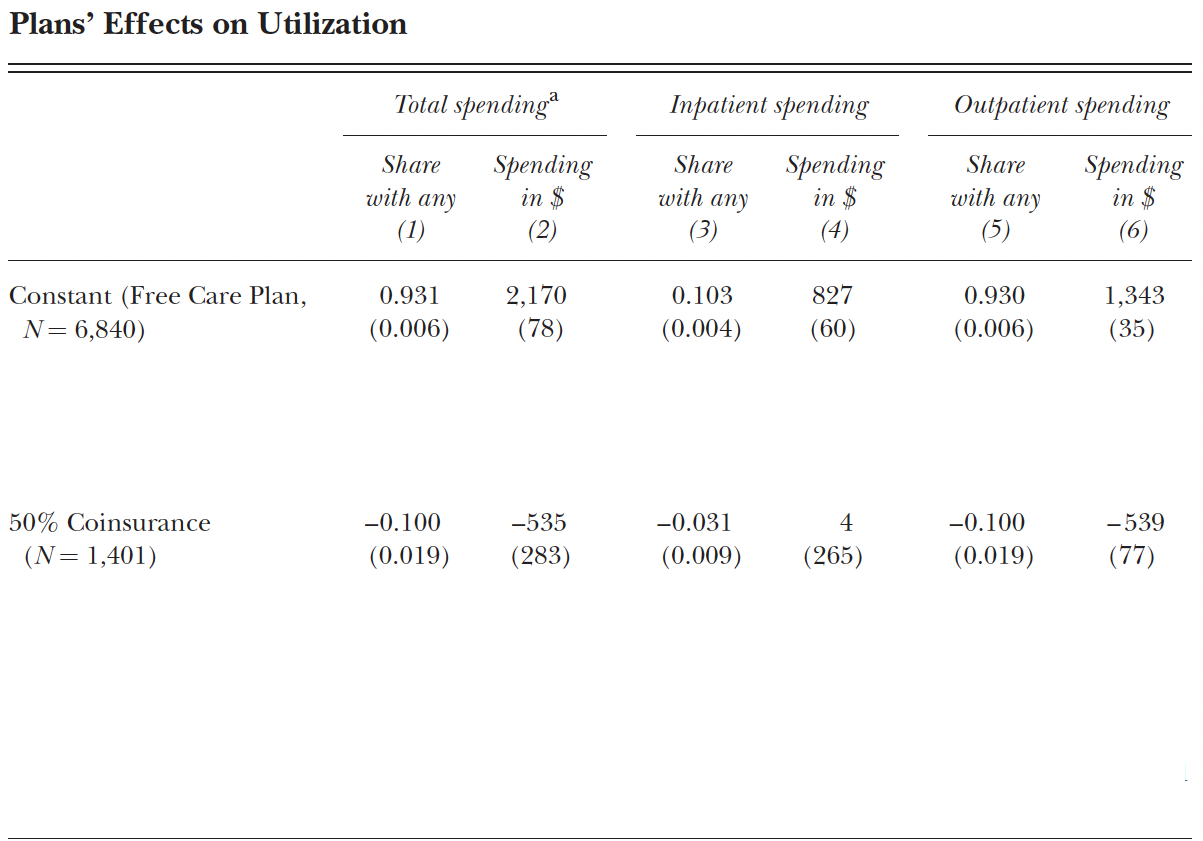
\includegraphics[scale=.53]{images/rand4.png}
    \end{center}
\end{frame}

\begin{frame}{Main Results}
    \begin{center}
        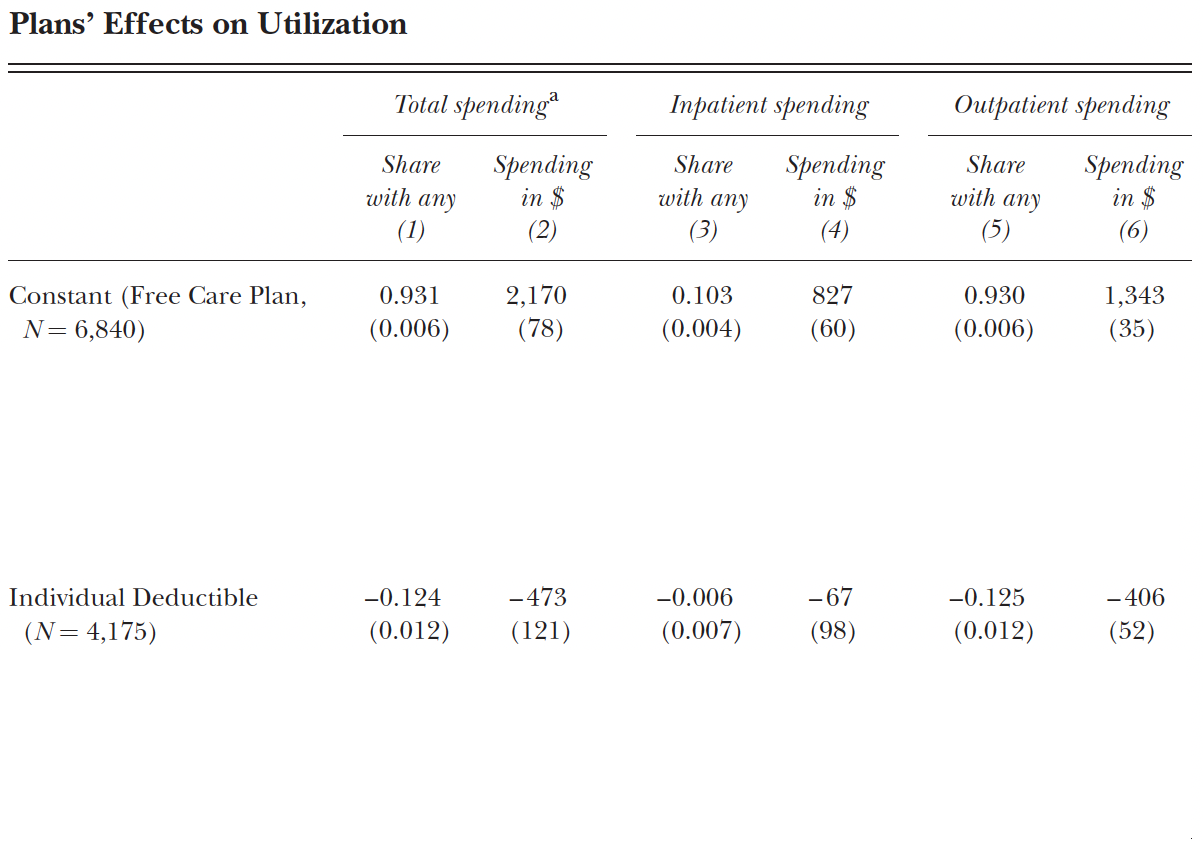
\includegraphics[scale=.53]{images/rand5.png}
    \end{center}
\end{frame}

\begin{frame}{Main Results}
    \begin{center}
        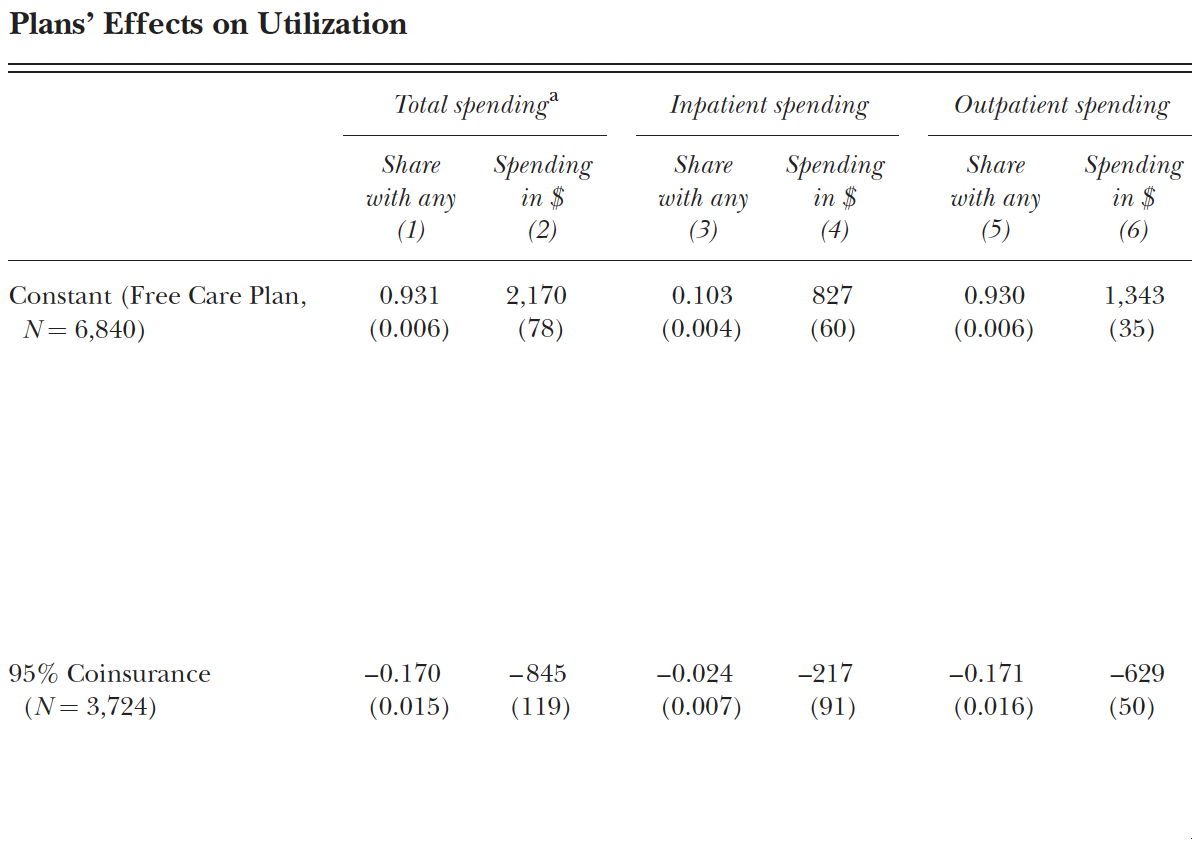
\includegraphics[scale=.53]{images/rand6.png}
    \end{center}
\end{frame}

\begin{frame}
\frametitle{The Oregon Health Insurance Experiment}

\begin{itemize}
  \item \textbf{Study Focus}: The Oregon Health Insurance Experiment (OHIE) examined the effects of a Medicaid expansion program targeting low-income adults not categorically eligible for traditional Medicaid program.\\\\[1em]

  \item \textbf{Eligibility Criteria}: To qualify, individuals needed to be aged 19 to 64, Oregon residents, U.S. citizens or legal immigrants, uninsured for six months, with income below the federal poverty level (e.g., \$10,400 for an individual in 2008), and have assets below \$2,000.\\\\[1em]

  \item \textbf{Program Details}: OHIE offered comprehensive medical benefits, including prescription drug coverage. It had no cost-sharing and low monthly premiums (ranging from \$0 to \$20, based on income), mainly provided through managed care organizations.\\\\[1em]
\end{itemize}
\end{frame}

\begin{frame}
\frametitle{The Oregon Health Insurance Experiment}

\begin{itemize}
  \item \textbf{Lottery Drawings}: Oregon conducted eight lottery drawings from a waiting list between March and September 2008. Individuals randomly selected by lottery, who met eligibility criteria upon application, were enrolled in the program.\\\\[1em]

  \item \textbf{Research Approval}: The Oregon Health Insurance Experiment had ethical approval from multiple institutional review boards.\\\\[1em]

  \item \textbf{Prior Findings}: Previous research found that Medicaid improved self-reported general health, reduced depression, and decreased financial strain. However, no statistically significant effects were observed on measured physical health (e.g., blood pressure, cholesterol, or glycated hemoglobin levels), employment, or earnings.\\\\[1em]

  \item \textbf{Effects on Healthcare Use}: Medicaid increased healthcare use, with improved access to primary care, prescription drugs, and preventive care. Notably, hospital use increased when measured from hospital administrative data, contrasting self-reported data.

\end{itemize}
\end{frame}


\begin{frame}{Main Results}
    \begin{center}
        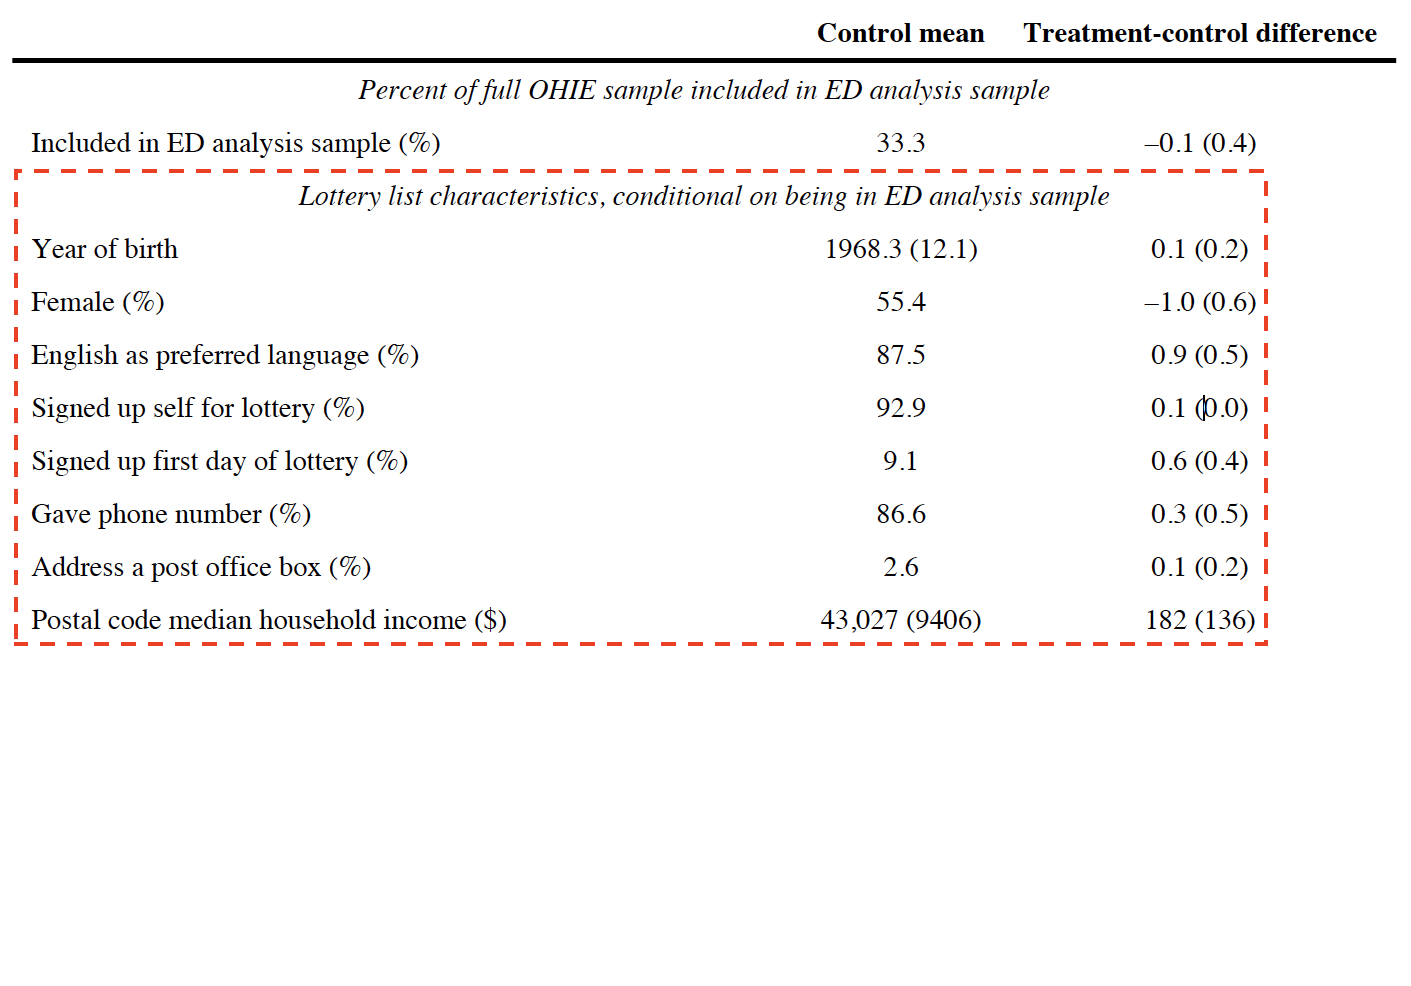
\includegraphics[scale=.6]{images/rand7.png}
    \end{center}
\end{frame}

\begin{frame}{Main Results}
    \begin{center}
        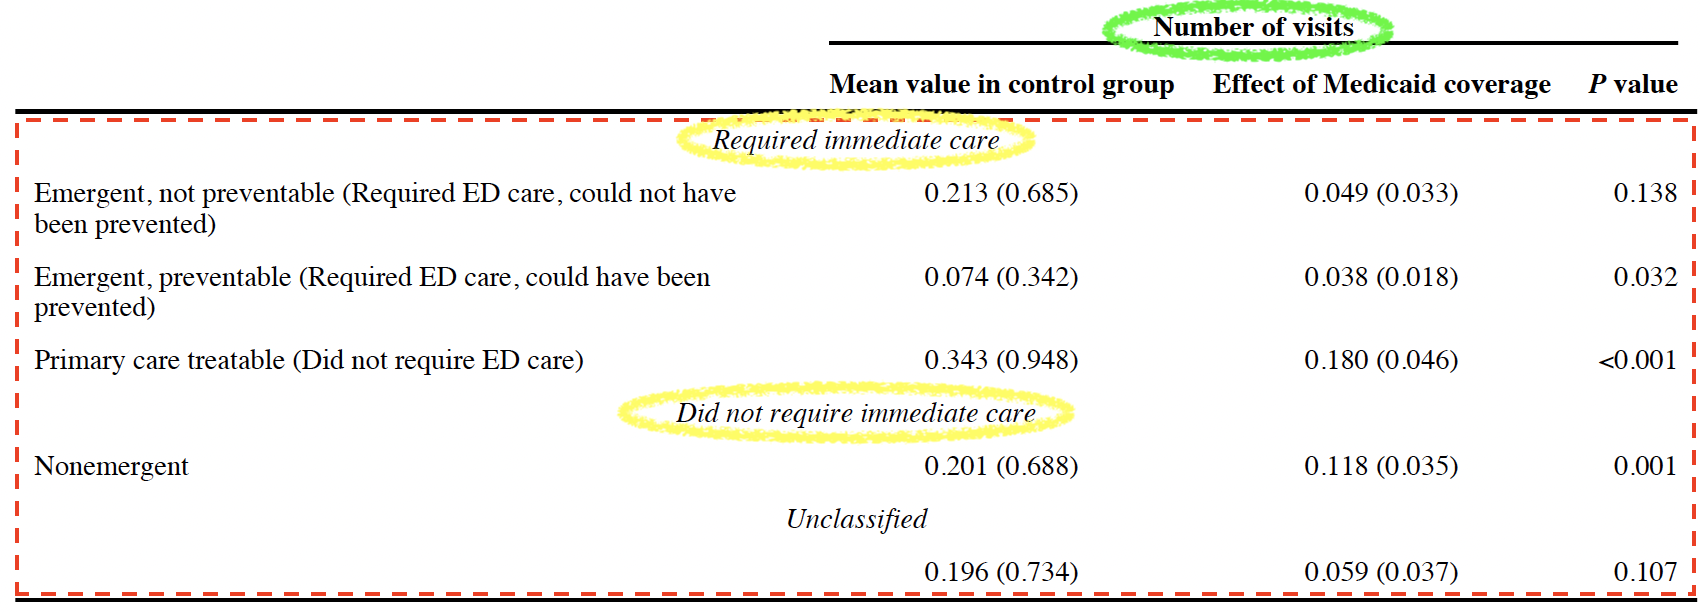
\includegraphics[scale=.5]{images/rand8.png}
    \end{center}
\end{frame}


\end{document}